% Part: model-theory
% Chapter: interpolation
% Section: separation

\documentclass[../../../include/open-logic-section]{subfiles}

\begin{document}

\olfileid{mod}{int}{sep}

\olsection{فصل الـ\printtoken{P}{sentence}}

لا بد قبل برهان الاستيفاء من تمهيد. مستوفية
$!A$ و$!B$ هي !!a{sentence}~$!C$ تحقق $!A \Entails !C$
و$!C \Entails !B$. والشرط الأخير يكافئ، بالمقابلة،
$\lnot !B \Entails \lnot !C$. فإذا كانت !!^a{sentence}~$!C$
على هذه الصفة قلنا إنها \emph{تفصل} $!A$ عن $\lnot !B$.
فطلب مستوفية لـ$!A$ و$!B$ هو طلب !!a{sentence}
تفصل $!A$ عن $\lnot !B$. ونوسّع النظر الآن إلى جملة
تفصل \emph{مجموعتين} من الـ!!{sentence}s، ففي هذا
التعميم نفع للبرهان.

\begin{defn}
\emph{تفصل} جملة~$!C$ مجموعتي الجمل ${\OLId{greek-variable}{Gamma}}$ و${\OLId{greek-variable}{Delta}}$ إذا وفقط إذا كان
${\OLId{greek-variable}{Gamma}} \Entails !C$ و${\OLId{greek-variable}{Delta}} \Entails \lnot !C$. وإذا لم توجد
!!{sentence} كهذه، كانت ${\OLId{greek-variable}{Gamma}}$ و${\OLId{greek-variable}{Delta}}$ \emph{غير قابلتين للفصل}.
\end{defn}

ويبيّن الشكل علاقات الاحتواء بين فئات نماذج ${\OLId{greek-variable}{Gamma}}$ و${\OLId{greek-variable}{Delta}}$ و$!C$:
\begin{figure}[h]
  \centering
  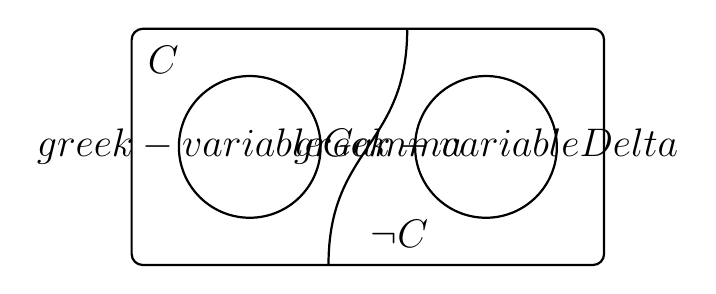
\begin{tikzpicture}[node distance=2cm, auto, thick]
    \draw [rounded corners] (0,0) -- (6,0) -- (6,3) -- (0,3) --  cycle;
    \draw (1.5,1.5) circle (0.9cm);
    \draw (4.5,1.5) circle (0.9cm);
    \path node at (1.5,1.5) {\Large ${\OLId{greek-variable}{Gamma}}$};
    \path node at (4.5,1.5) {\Large ${\OLId{greek-variable}{Delta}}$};
    \path node at (0.4,2.6) {\Large $\formula{C}$};
    \path node at (3.4,0.4) {\Large $\lnot \formula{C}$};
    \draw (2.5,0) .. controls (2.5,1.5) and (3.5,1.5) .. (3.5,3);
  \end{tikzpicture}
  \caption{$!C$ تفصل ${\OLId{greek-variable}{Gamma}}$ عن ${\OLId{greek-variable}{Delta}}$}
  \ollabel{fig:sep}
\end{figure}


\begin{lem}\ollabel{lem:sep1}
افترض أن $\Lang{L}_{\OLMathNumeral{0}}$ هي اللغة التي تحتوي كل !!{constant} و!!{function}
و!!{predicate} (عدا~$\doteq$) يقع في ${\OLId{greek-variable}{Gamma}}$ و${\OLId{greek-variable}{Delta}}$ \emph{معًا}،
ولتكن $\Lang{L}'_{\OLMathNumeral{0}}$ ناتجة بإضافة عدد لا نهائي من الـ!!{constant}s الجديدة
$\Obj c_{\OLId{latin-ordinary}{n}}$، حيث ${\OLId{latin-ordinary}{n}} \ge {\OLMathNumeral{0}}$. إذا كانت ${\OLId{greek-variable}{Gamma}}$ و${\OLId{greek-variable}{Delta}}$ غير قابلتين
للفصل في $\Lang{L}_{\OLMathNumeral{0}}$، فهما غير قابلتين للفصل في $\Lang{L}'_{\OLMathNumeral{0}}$ أيضًا.
\end{lem}

\begin{proof}
لنفرض خلاف المطلوب: أن ${\OLId{greek-variable}{Gamma}}$ و${\OLId{greek-variable}{Delta}}$ تفصلهما
جملة في $\Lang{L}'_{\OLMathNumeral{0}}$. فيكون
${\OLId{greek-variable}{Gamma}} \Entails \Subst{!C}{{\OLId{latin-ordinary}{c}}}{{\OLId{latin-ordinary}{x}}}$ و
${\OLId{greek-variable}{Delta}} \Entails \lnot \Subst{!C}{{\OLId{latin-ordinary}{c}}}{{\OLId{latin-ordinary}{x}}}$ لبعض
$!C \in \Lang{L}_{\OLMathNumeral{0}}$، حيث ${\OLId{latin-ordinary}{c}}$~!!{constant} جديد.
ونقتصر على هذه الحال؛ أما ما ينتج من $!C$ باستعمال أكثر
من !!{constant} جديد فبرهانه نظيرها.
بالتراص نجد جزءًا \emph{منتهيًا} ${\OLId{greek-variable}{Gamma}}_{\OLMathNumeral{0}}$ من ${\OLId{greek-variable}{Gamma}}$
وجزءًا منتهيًا ${\OLId{greek-variable}{Delta}}_{\OLMathNumeral{0}}$ من ${\OLId{greek-variable}{Delta}}$، بحيث
${\OLId{greek-variable}{Gamma}}_{\OLMathNumeral{0}} \Entails \Subst{!C}{{\OLId{latin-ordinary}{c}}}{{\OLId{latin-ordinary}{x}}}$ و
${\OLId{greek-variable}{Delta}}_{\OLMathNumeral{0}} \Entails \lnot \Subst{!C}{{\OLId{latin-ordinary}{c}}}{{\OLId{latin-ordinary}{x}}}$.
نجعل $!G$ اقتران الـ!!{formula}s التي في ${\OLId{greek-variable}{Gamma}}_{\OLMathNumeral{0}}$،
و$!H$ اقتران الـ!!{formula}s التي في ${\OLId{greek-variable}{Delta}}_{\OLMathNumeral{0}}$، فنحصل على
\begin{align*}
  !G & \Entails \Subst{!C}{{\OLId{latin-ordinary}{c}}}{{\OLId{latin-ordinary}{x}}}, & !H  \Entails \lnot \Subst{!C}{{\OLId{latin-ordinary}{c}}}{{\OLId{latin-ordinary}{x}}}.
\end{align*}
من الجهة الأولى نستنتج بالتعميم $!G \Entails \lforall[{\OLId{latin-ordinary}{x}}][!C]$.
ومن الجهة الثانية نستنتج بالمقابلة
$\Subst{!C}{{\OLId{latin-ordinary}{c}}}{{\OLId{latin-ordinary}{x}}} \Entails \lnot !H$، فيلزم
$\lforall[{\OLId{latin-ordinary}{x}}][!C] \Entails \lnot !H$.
وبمقابلة أخرى نحصل على $!H \Entails \lnot \lforall[{\OLId{latin-ordinary}{x}}][!C]$.
ثم تقضي الرتابة بأن
\begin{align*}
  {\OLId{greek-variable}{Gamma}} &\Entails \lforall[{\OLId{latin-ordinary}{x}}][!C], &
  {\OLId{greek-variable}{Delta}} & \Entails \lnot \lforall[{\OLId{latin-ordinary}{x}}][!C],
\end{align*}
فتكون $\lforall[{\OLId{latin-ordinary}{x}}][!C]$ فاصلةً بين~${\OLId{greek-variable}{Gamma}}$ و${\OLId{greek-variable}{Delta}}$ في $\Lang{L}_{\OLMathNumeral{0}}$، خلاف الفرض.
\end{proof}

\begin{lem}\ollabel{lem:sep2}
افترض أن ${\OLId{greek-variable}{Gamma}} \cup \{ \lexists[{\OLId{latin-ordinary}{x}}][!S] \}$ و${\OLId{greek-variable}{Delta}}$ غير قابلتين
للفصل، وأن ${\OLId{latin-ordinary}{c}}$~!!{constant} جديد لا يقع في ${\OLId{greek-variable}{Gamma}}$ أو ${\OLId{greek-variable}{Delta}}$ أو
$!S$. عندئذ تكون
${\OLId{greek-variable}{Gamma}} \cup \{ \lexists[{\OLId{latin-ordinary}{x}}][!S], \Subst{!S}{{\OLId{latin-ordinary}{c}}}{{\OLId{latin-ordinary}{x}}} \}$ و${\OLId{greek-variable}{Delta}}$
غير قابلتين للفصل أيضًا.
\end{lem}

\begin{proof}
لنفرض أن $!C$ تفصل
${\OLId{greek-variable}{Gamma}} \cup \{\lexists[{\OLId{latin-ordinary}{x}}][!S], \Subst{!S}{{\OLId{latin-ordinary}{c}}}{{\OLId{latin-ordinary}{x}}}\}$ عن ${\OLId{greek-variable}{Delta}}$،
مع أن ${\OLId{greek-variable}{Gamma}} \cup \{\lexists[{\OLId{latin-ordinary}{x}}][!S] \}$ و${\OLId{greek-variable}{Delta}}$
غير قابلتين للفصل. والبحث على حالين:
\begin{enumerate}
\item إن لم يقع ${\OLId{latin-ordinary}{c}}$ في $!C$، كانت
  ${\OLId{greek-variable}{Gamma}} \cup \{\lexists[{\OLId{latin-ordinary}{x}}][!S], \lnot!C \}$ قابلة للإرضاء؛
  وإلا فصلت $!C$~${\OLId{greek-variable}{Gamma}} \cup \{\lexists[{\OLId{latin-ordinary}{x}}][!S] \}$ عن ${\OLId{greek-variable}{Delta}}$.
  ولنا أن نضيف $\Subst{!S}{{\OLId{latin-ordinary}{c}}}{{\OLId{latin-ordinary}{x}}}$ ونبقي الإرضاء، بتأويل
  الثابت الجديد بشاهد الوجود. فلا تفصل $!C$
  المجموعة ${\OLId{greek-variable}{Gamma}} \cup \{ \lexists[{\OLId{latin-ordinary}{x}}][!S], \Subst{!S}{{\OLId{latin-ordinary}{c}}}{{\OLId{latin-ordinary}{x}}} \}$
  عن ${\OLId{greek-variable}{Delta}}$، خلاف الفرض.
\item وإن وقع ${\OLId{latin-ordinary}{c}}$ في $!C$، كتبنا $!C$ على الصورة
  $\Subst{!C}{{\OLId{latin-ordinary}{c}}}{{\OLId{latin-ordinary}{x}}}$. وعندئذ
  \[
  {\OLId{greek-variable}{Gamma}} \cup \{ \lexists[{\OLId{latin-ordinary}{x}}][!S], \Subst{!S}{{\OLId{latin-ordinary}{c}}}{{\OLId{latin-ordinary}{x}}}\} \Entails \Subst{!C}{{\OLId{latin-ordinary}{c}}}{{\OLId{latin-ordinary}{x}}},
  \]
  فنستنتج ${\OLId{greek-variable}{Gamma}}, \lexists[{\OLId{latin-ordinary}{x}}][!S] \Entails \lforall[{\OLId{latin-ordinary}{x}}][(!S \lif !C)]$
  بمبرهنة الاستنباط والتعميم، ثم
  ${\OLId{greek-variable}{Gamma}} \cup \{ \lexists[{\OLId{latin-ordinary}{x}}][!S] \} \Entails \lexists[{\OLId{latin-ordinary}{x}}][!C]$.
  وفي الجهة الأخرى ${\OLId{greek-variable}{Delta}} \Entails \lnot \Subst{!C}{{\OLId{latin-ordinary}{c}}}{{\OLId{latin-ordinary}{x}}}$،
  فيعطي التعميم ${\OLId{greek-variable}{Delta}} \Entails \lnot \lexists[{\OLId{latin-ordinary}{x}}][!C]$.
  فتكون ${\OLId{greek-variable}{Gamma}} \cup \{\lexists[{\OLId{latin-ordinary}{x}}][!S] \}$ و${\OLId{greek-variable}{Delta}}$
  قابلتين للفصل، وهذا تناقض.
\end{enumerate}
\end{proof}

\end{document}
